\chapter{Experimentálna časť}


\section {Ciele experimentu}

V oblasti Q-learning algoritmoch je možné pozorovať dva hlavné smery výskumu

\begin{itemize}
\item aproximácia funkcie ohodnotení \cite{bib:aproximation_01} \cite{bib:aproximation_02} \cite{bib:aproximation_03} \cite{bib:aproximation_04}
\item spôsob výberu akcie \cite{bib:strategy_01} \cite{bib:strategy_02} \cite{bib:strategy_03}
\end{itemize}

Obe majú široké pole diskusií v snahe vyriešit niekoľko hlavných problémov Q-learning
algoritmu a to najmä :

\begin{itemize}
\item veľký počet prechodov medzi stavmi
\item malá zmena vo výpočte $Q(s(n),a(n))$ môže spôsobiť veľké zmeny v stratégií.
\end{itemize}

Cieľom práce je na danej množine odmeňovacích funkcií $R(s(n), a(n))$ overiť
možnosti aproximácie $Q(s(n), a(n))$. Prvým intuitivným spôsobom bola snaha aproximovať
predmentnú funkciu doprednými neurónovými sieťami. Principiálne tomu nič nebráni,
problém je ale nedokonalý algoritmus učenia, a to, že sa vplyvom rekurentnej povahy
Q-learning algoritmu pokúša neurónová sieť zároveň predikovať správnu hodnotu
a zároveň učiť na požadovanú hodnotu.

\begin{figure}[!htb]
\center
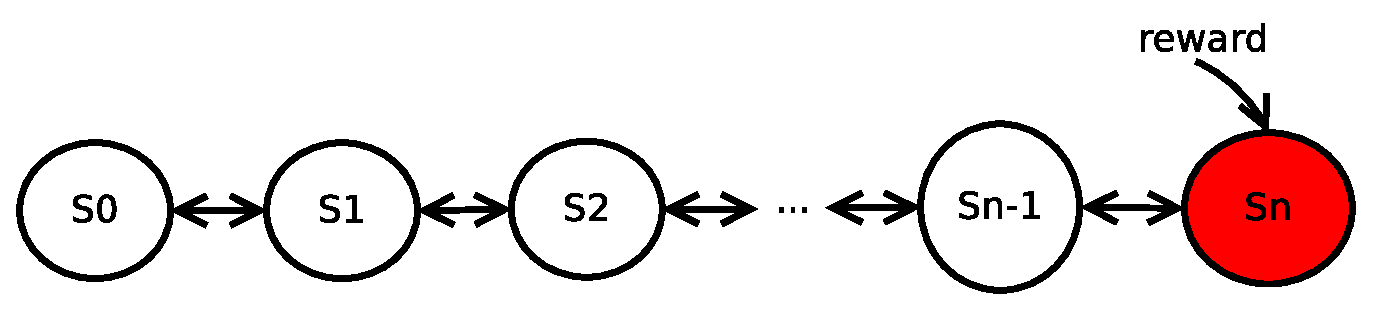
\includegraphics[scale=.4]{../diagrams/q_chain_problem.eps}
\caption{Ilustrácia postupného nabaľovania chyby}
\label{img:snowball_problem}
\end{figure}

Postupne sa tak v sieti nabaľuje chyba. Tento problém ilustruje \ref{img:snowball_problem}.
Je daná postupnosť stavov a každom okrem východzieho a cieľového sú dve akcie.
Odmena $R(s,a)$ je všade nulová, len po dosiahnutí cieľového stavu je rovná kladnej hodnote.

Pre korektné vyplnenie hodnôt v $s_{n-1}$ sa vyžaduje korektá hodnota v $s_{n}$

\begin{align*}
    Q(s(1),a(1)) &= R(s(1),a(1)) + \gamma \max_{a(0) \in \mathbb{A}} Q(s(0), a(0)) \\
    Q(s(2),a(2)) &= R(s(2),a(2)) + \gamma \max_{a(1) \in \mathbb{A}} Q(s(1), a(1)) \\
    & \dots
\end{align*}

V prípade doprednej siete učenej algoritmom Backpropagation, zmena hodnoty v jednom bode $Q(s(n),a(n))$ spôsobí
zmenu vo všetkých ostatných hodnotách a nikde nie je zaručené, že k správnej hodnote -
v určitom štádiu učenia sa tak môže zdať, že hodnoty koretkne kovergujú, a inom
sa môžu vzďaľovať. Práve preto sa pre klasické úlohy rozpoznávania predkladajú sieti vzory
v náhodonom poradí a v mnohých opakovaniach. Vzory a požadované výstupy sú však nezávislé.

\subsection{Divergencia riešenia}

Tento efekt divergencie bol pozrovaný nie len vyššie uvedenými autormi, ale aj experimentálne
overený v tejto práci. Usporiadanie experimentu je na obrázku \ref{img:1D_experiment_schem}.
Robot má dve akcie, pohyb o pevne zvolený krkok vľavo alebo vpravo. Úlohou je dostať sa
do cieľa, ktorý môže byť umiestnený kdekoľvek. Pre jednoduchosť bol vybraný dvoj rozmerný stavový priestor
z rozsahu $s \in \langle -1, 1 \rangle$. Stav systému charakterizovaný vektorom $s$ je
poloha robota voči počiatku a poloha cieľa voči počiatku, takýto systém je aj dobre graficky znázorniteľný.

\begin{figure}[!htb]
\center
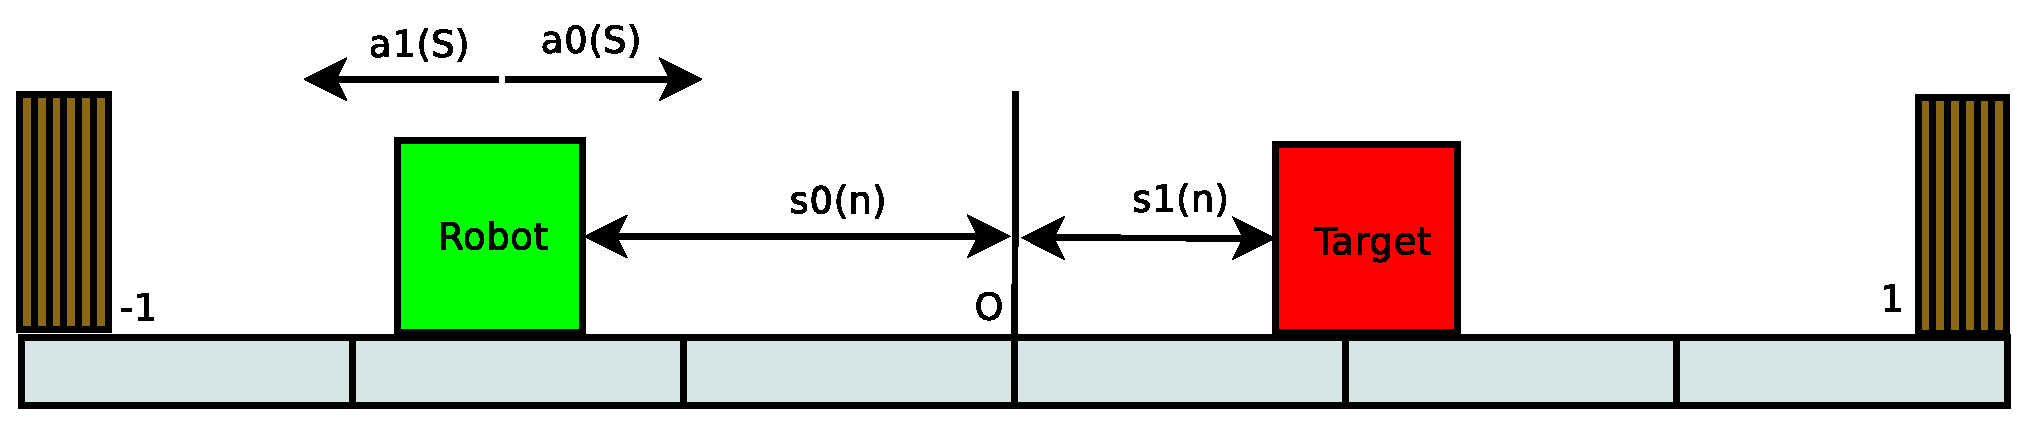
\includegraphics[scale=.3]{../diagrams/1D_robot_diagram.eps}
\caption{Schéma experimentu pre doprednú neurónovú sieť}
\label{img:1D_experiment_schem}
\end{figure}

Z ostatných parametrov ktoré boli použité pre beh experimentu :

\begin{itemize}
\item počet iterácií = 10000000
\item delenie stavového priestoru = 1/8.0
\item $\gamma = 0.7$
\item neurónová sieť :
  \begin{itemize}
  \item počet skrytých vrstiev = 2
  \item počet neurónov v skrytých vrstvách = 10
  \item rozsha váh = 4.0
  \item krok učenia $\eta = 0.001$
  \end{itemize}
\end{itemize}

Najskôr bolo určené riešenie použitím tabuľky (ktoré bolo pre malý počet stavov možné spočítať).
Najdôležitejší výstup je výber korektnej akcie, kde $+1$ znamená jeden smer a $-1$ smer opačný.
Veľmi ľahko sa dá očakávať ostré rozdelenie stavového priestoru po diagonále :
ak je robot naľavo od cieľa musí sa pohybovať doprava a naopak. Výsledok je na obrázku
\ref{img:divergence_table_action}. Pre úplnosť, obrázok \ref{img:divergence_table_q_map}
znázorňuje hodnoty $\max_{a(n-1) \in \mathbb{A}} Q(s, a)$. Opäť sa dá ľahko očakávať
že pre najmenšiu vzdialenosť bude táto hodnota najväčšia - hodnoty na diagonále.


\begin{figure}[!htb]
\centering
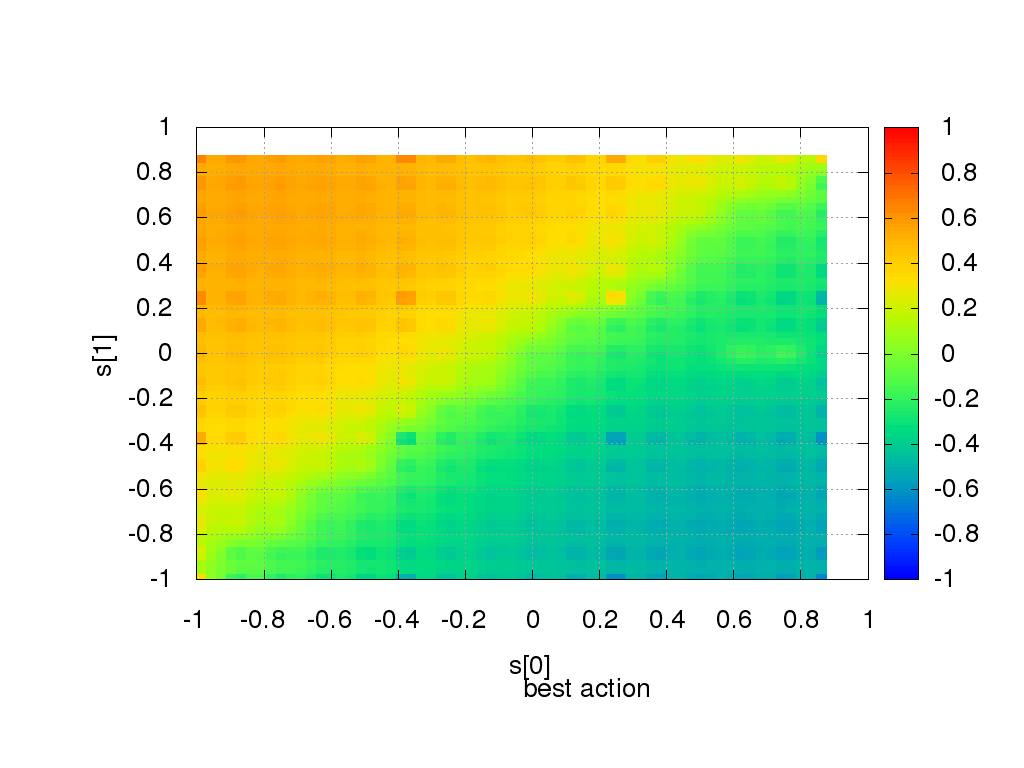
\includegraphics[scale=.4]{../../results_q_learning/experiment_divergence/table/q_action.png}
\caption{Najlepšia akcia pre riešenie s tabuľkou}
\label{img:divergence_table_action}
\end{figure}


\begin{figure}[!htb]
\centering
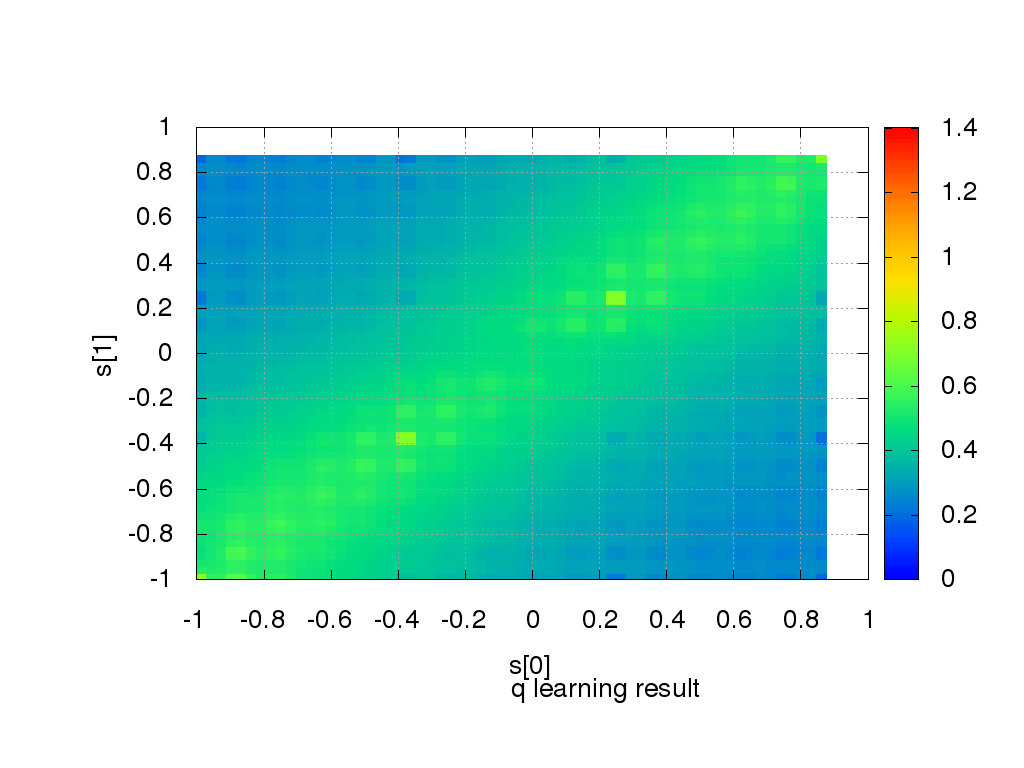
\includegraphics[scale=.4]{../../results_q_learning/experiment_divergence/table/q_map.png}
\caption{Hodnoty $\max_{a(n-1) \in \mathbb{A}} Q(s, a)$ pre riešenie s tabuľkou}
\label{img:divergence_table_q_map}
\end{figure}

Jedno z najlepších riešení dosiahnuté doprednou neurónovou sieťou učenou
Backpropagation algoritmom je na obrázkoch \ref{img:divergence_table_action} a
\ref{img:divergence_table_q_map}.


\begin{figure}[!htb]
\centering
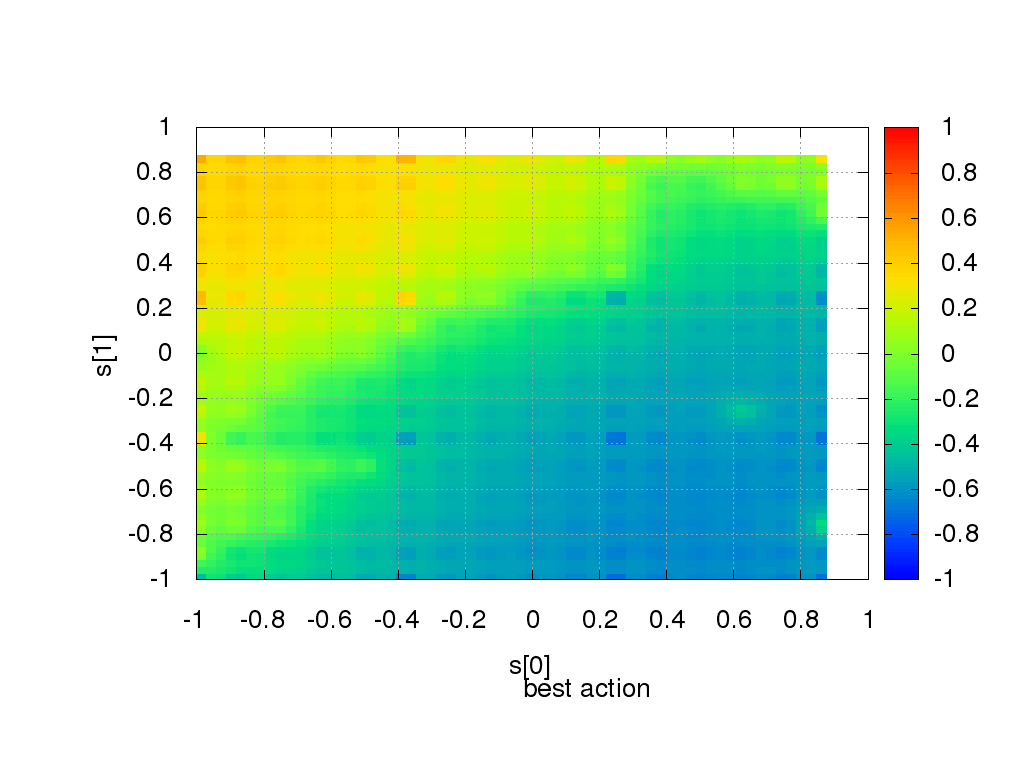
\includegraphics[scale=.4]{../../results_q_learning/experiment_divergence/testing_neuron/q_action.png}
\caption{Najlepšia akcia pre riešenie s neurónovou sieťou}
\label{img:divergence_table_action}
\end{figure}


\begin{figure}[!htb]
\centering
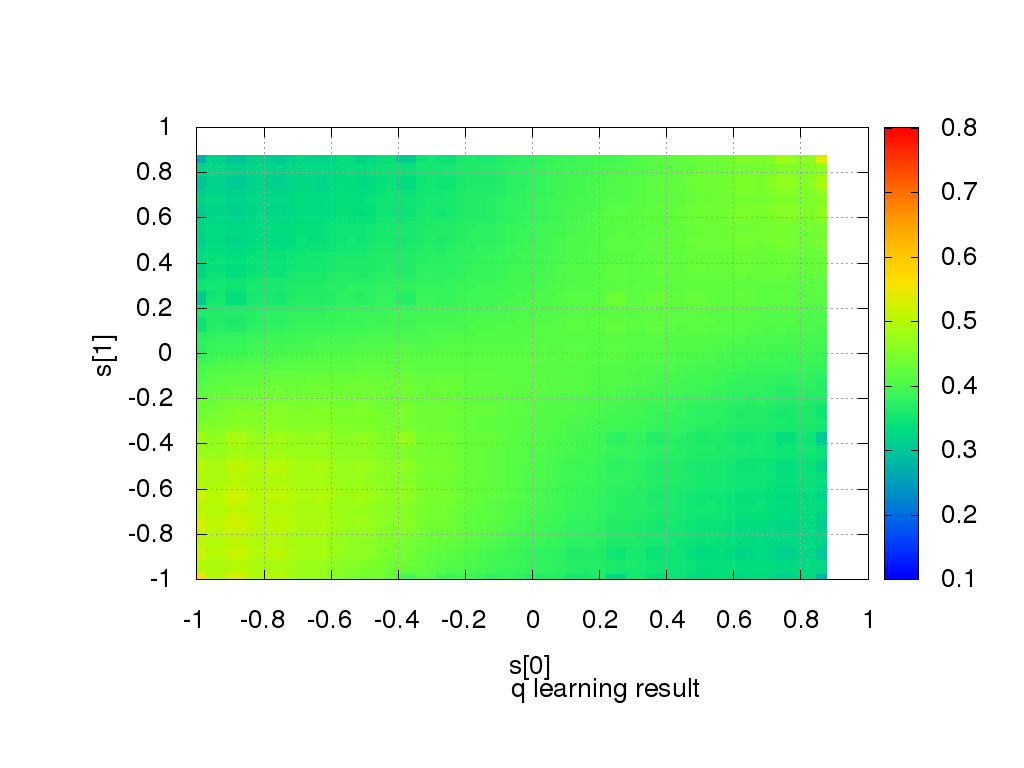
\includegraphics[scale=.4]{../../results_q_learning/experiment_divergence/testing_neuron/q_map.png}
\caption{Hodnoty $\max_{a(n-1) \in \mathbb{A}} Q(s, a)$ pre riešenie s neurónovou sieťou}
\label{img:divergence_table_q_map}
\end{figure}

Napriek jednoduchej úlohe, nie je možné povedať že sieť úspešne aproximuje tento problém.
Porovnaním výstupov najlepších akcií je možné vidieť určitý náznak podobnosti, ktorý je
však vzhľadom na irelevantnosť úlohy bezpredmentný a dosahuje priveľkú chybu, najmä
ak sa robot už blížil k cieľu.

Najlepšie výsledky dosahovala dopredná neurónová sieť s novo zavedeným modelom
neurónu v tvare

\begin{equation}
y(x(n)) = tanh(\sum\limits_{i=0}^{N-1} w_ix_i(n) + \sum\limits_{j=0}^{N-1} \sum\limits_{i=0}^{j} v_{ij}x_i(n)x_j(n))
\label{eq:neuron_model}
\end{equation}

kde
x(n) je vstup do neurónu \\
w je vektor váh \\
v je matica váh \\

Takto definovaný model neurónu umožňuje okrem bežných funkcí McCuloh-Pittsovho neurónu aj násobiť
prvky vstupného vektora (časť $v_{ij}x_i(n)x_j(n)$). Dôsledkom toho je realizácia zložitých
funkcií len s použitím jednej skrytej vrstvy - výrazne sa tak zjednoduší učenie. Medzi typické
funkcie ktoré sa s McCuloh-Pittsovim neurónom a jendou skytou vrstvou ťažko realizujú, možno uviesť napr :
Fourierova transformácia, zmiešavanie signálov, riadenie toku dát na základe inej časti dát.
Najmä posledne uvedená zvyšuje stupeň abstrakcie, kde neurónová sieť neaproximuje len jeden
naučený druh funkcie, ale môže aproximovať viac, úplne rozdielných a medzi nimi vyberať.
Uvedený model bol doteraz nepublikovaný v inej literatúre.



\section {Riešenie aproximácie}

Uvedení autori najčastejšie používajú tzv. príznaky (features) na aproximovanie $Q(s(n), a(n))$
\begin{align}
Q(s(n), a(n)) = \sum\limits_{j=1} w_j g_j(s(n), a(n))
\label{eq:features_func}
\end{align}

kde $g_j(s(n), a(n))$ sú funkcie príznakov, ktorých je konečný počet a
$w_j$ predstavuje váhy ich lineárnej kombinácie.

Príznaky sú funkcie, ktoré sú pevne zvolené a závisia od typu úlohy. Práve to predstavuje najväčší
nedostatok. Cieľom navrhovaného experimentu je využiť príznaky ktorých parametre
sa menia - bázické funkcie. Vzniká tak akýsi hybrid medzi neurónovou sieťou a lineárnou kombináciou
pevne zvolených príznakov.

Z ohľadom na minimalizovanie vplyvu zmeny parametrov j-teho príznaku alebo váhy $w_j$
na ostatné príznaky a váhy, je potrebné, aby ich bolo možné nastavovať nezávislé -
aby vhodná séria príznakov pokryla svoju podmonožinu stavového priestoru. Toto
je možné dosiahnuť ortogonalitou príznakou, stráca sa však možnosť generovať funkciu
ako je lineárna kombinácia týchto ortogonálnych funkcií. Vhodným kompromisom sú
preto funkcie uvedené v \ref{eq:basis_functions_01}, alebo funkcia \ref{eq:peak_hill}.


\section {Návrh experimentu}

V niekoľkých bodoch je možné postup určiť ako

\begin{itemize}
\item výber funkcií $R(s(n), a(n))$
\item určenie presného riešenia, použitím tabuľky s veľkým počtom prvkov
\item voľba aproximačnej metódy
\item pre každú $R(s(n), a(n))$ spočítať niekoľko nezávislych behov
\item výsledky porovnať s presným riešením, overiť a zosumarizovať
\end{itemize}

Funkcie $R(s(n), a(n))$ budu vybrané tak aby boli riedke a plne sa využil Q-learing -
okamžité odmeny sú známe len v malom počte prípadov.
Postupne sa obmenia pre rôzne počty nenulových prvkov.

Presné riešenie, aby bolo možné spočítať bude mať niekoľko tisíc diskrétnych stavov.
Pre jednoduchosť, bude v každom stave rovnaká a presne definovaná množina akcií.

Vyberie sa niekoľko aproximačných metód, ktoré sa použijí na spočítanie $Q(s(n), a(n))$.
Tu je nevyhnutné upozorniť na častú metodickú chybu : aj keď je možné $Q(s(n), a(n))$
spočítať presne, nesmie byť toto presne riešenie použité na stanovenie približného riešenia.
Príkladom je dopredná neurónová sieť, ktorá sa dá veľmi ľahko natrénovať ak je množina požadovaných
výstupov vopred známa. V prípade Q-learning algoritmu sa ale požadované hodnoty spočítavajú
rekuretne, až počas behu.

Kedže voľba niektorých počiatočných parametrov aproximačných metód je náhodná,
je nevyhnutné spočítať niekoľko nezávislých behov a overť tak rozptyl, minimálnu, maximálnu
a priemernu chybu.


Aby sa dalo kvalitatívne ohodnotiť použité riešenie, je nutné urobiť veľký počet experimentov.
Aby bolo možné ľahko graficky znázorniť výsledok, bude stavový priestor dvojrozmerný a platí
$s(n) \in \langle -1, 1 \rangle$.
Agent si bude vyberať z pevne danej množiny akcií a bude sa tak v tomto priestore môcť pohybovať a to :

$\mathbb{A} = [ [0, 1], [0, -1], [1,  0], [-1, 0], [1, -1], [1, 1], [-1, -1], [-1, 1]] $

prostredie umožní zmenu stavu vykonaním akcie $a(n) \in \mathbb{A}$, a to podľa

\begin{equation}
s(n+1) = s(n) + a(n){dt}
\label{eq:q_learning_next_state}
\end{equation}

Jednotlivé funkcie $R^k(s(n), a(n))$ predstavujú mapy odmien v ktorých sa agent pohybuje. Pre zjednodušenie
bude platiť, že nezáleží ktorou akciou sa agent dostal do daného stavu - funkcia bude
mať teda tvar $R^k(s(n))$ a predstavuje teda odmenu za to, že sa agent dostal na nejaké miesto.

Ako metódy aprximácie je zvolených 6 rôznych funkcií.

\begin{enumerate}
\item riedka tabuľka
\item Gaussova krivka $f_j^1(\boldmath{s(n), a(n)})$ \ref{eq:basis_functions}
\item Gaussova krivka $f_j^1(\boldmath{s(n), a(n)})$ kombinovaná s riedkou tabuľkou
\item Modifikácia Kohonenovej neurónovej siete $f_j^2(\boldmath{s(n), a(n)})$
\item Modifikácia Kohonenovej neurónovej siete $f_j^2(\boldmath{s(n), a(n)})$ s riedkou tabuľkou
\item Guassova krivka a adaptívna tabuľka \ref{eq:peak_hill}
\end{enumerate}

Pre každú z nich prebehne 20 trialov aby bolo možné urobiť štatistické vyhodnotenie.
V každom trialy prebehne 10*50000 učiacich interácií aby bolo možné v 10 tich krokoch sledovať
priebeh učenia. Na konci prebehne 50 behov agentov z náhodných východzich stavov aby bolo
možné sledovať ich cestu stavovým priestorom. Spolu teda prebehne 560 nezávislých experimentov
a celkovo 280mil. behu algortimu.

\begin{figure}[!htb]
\center
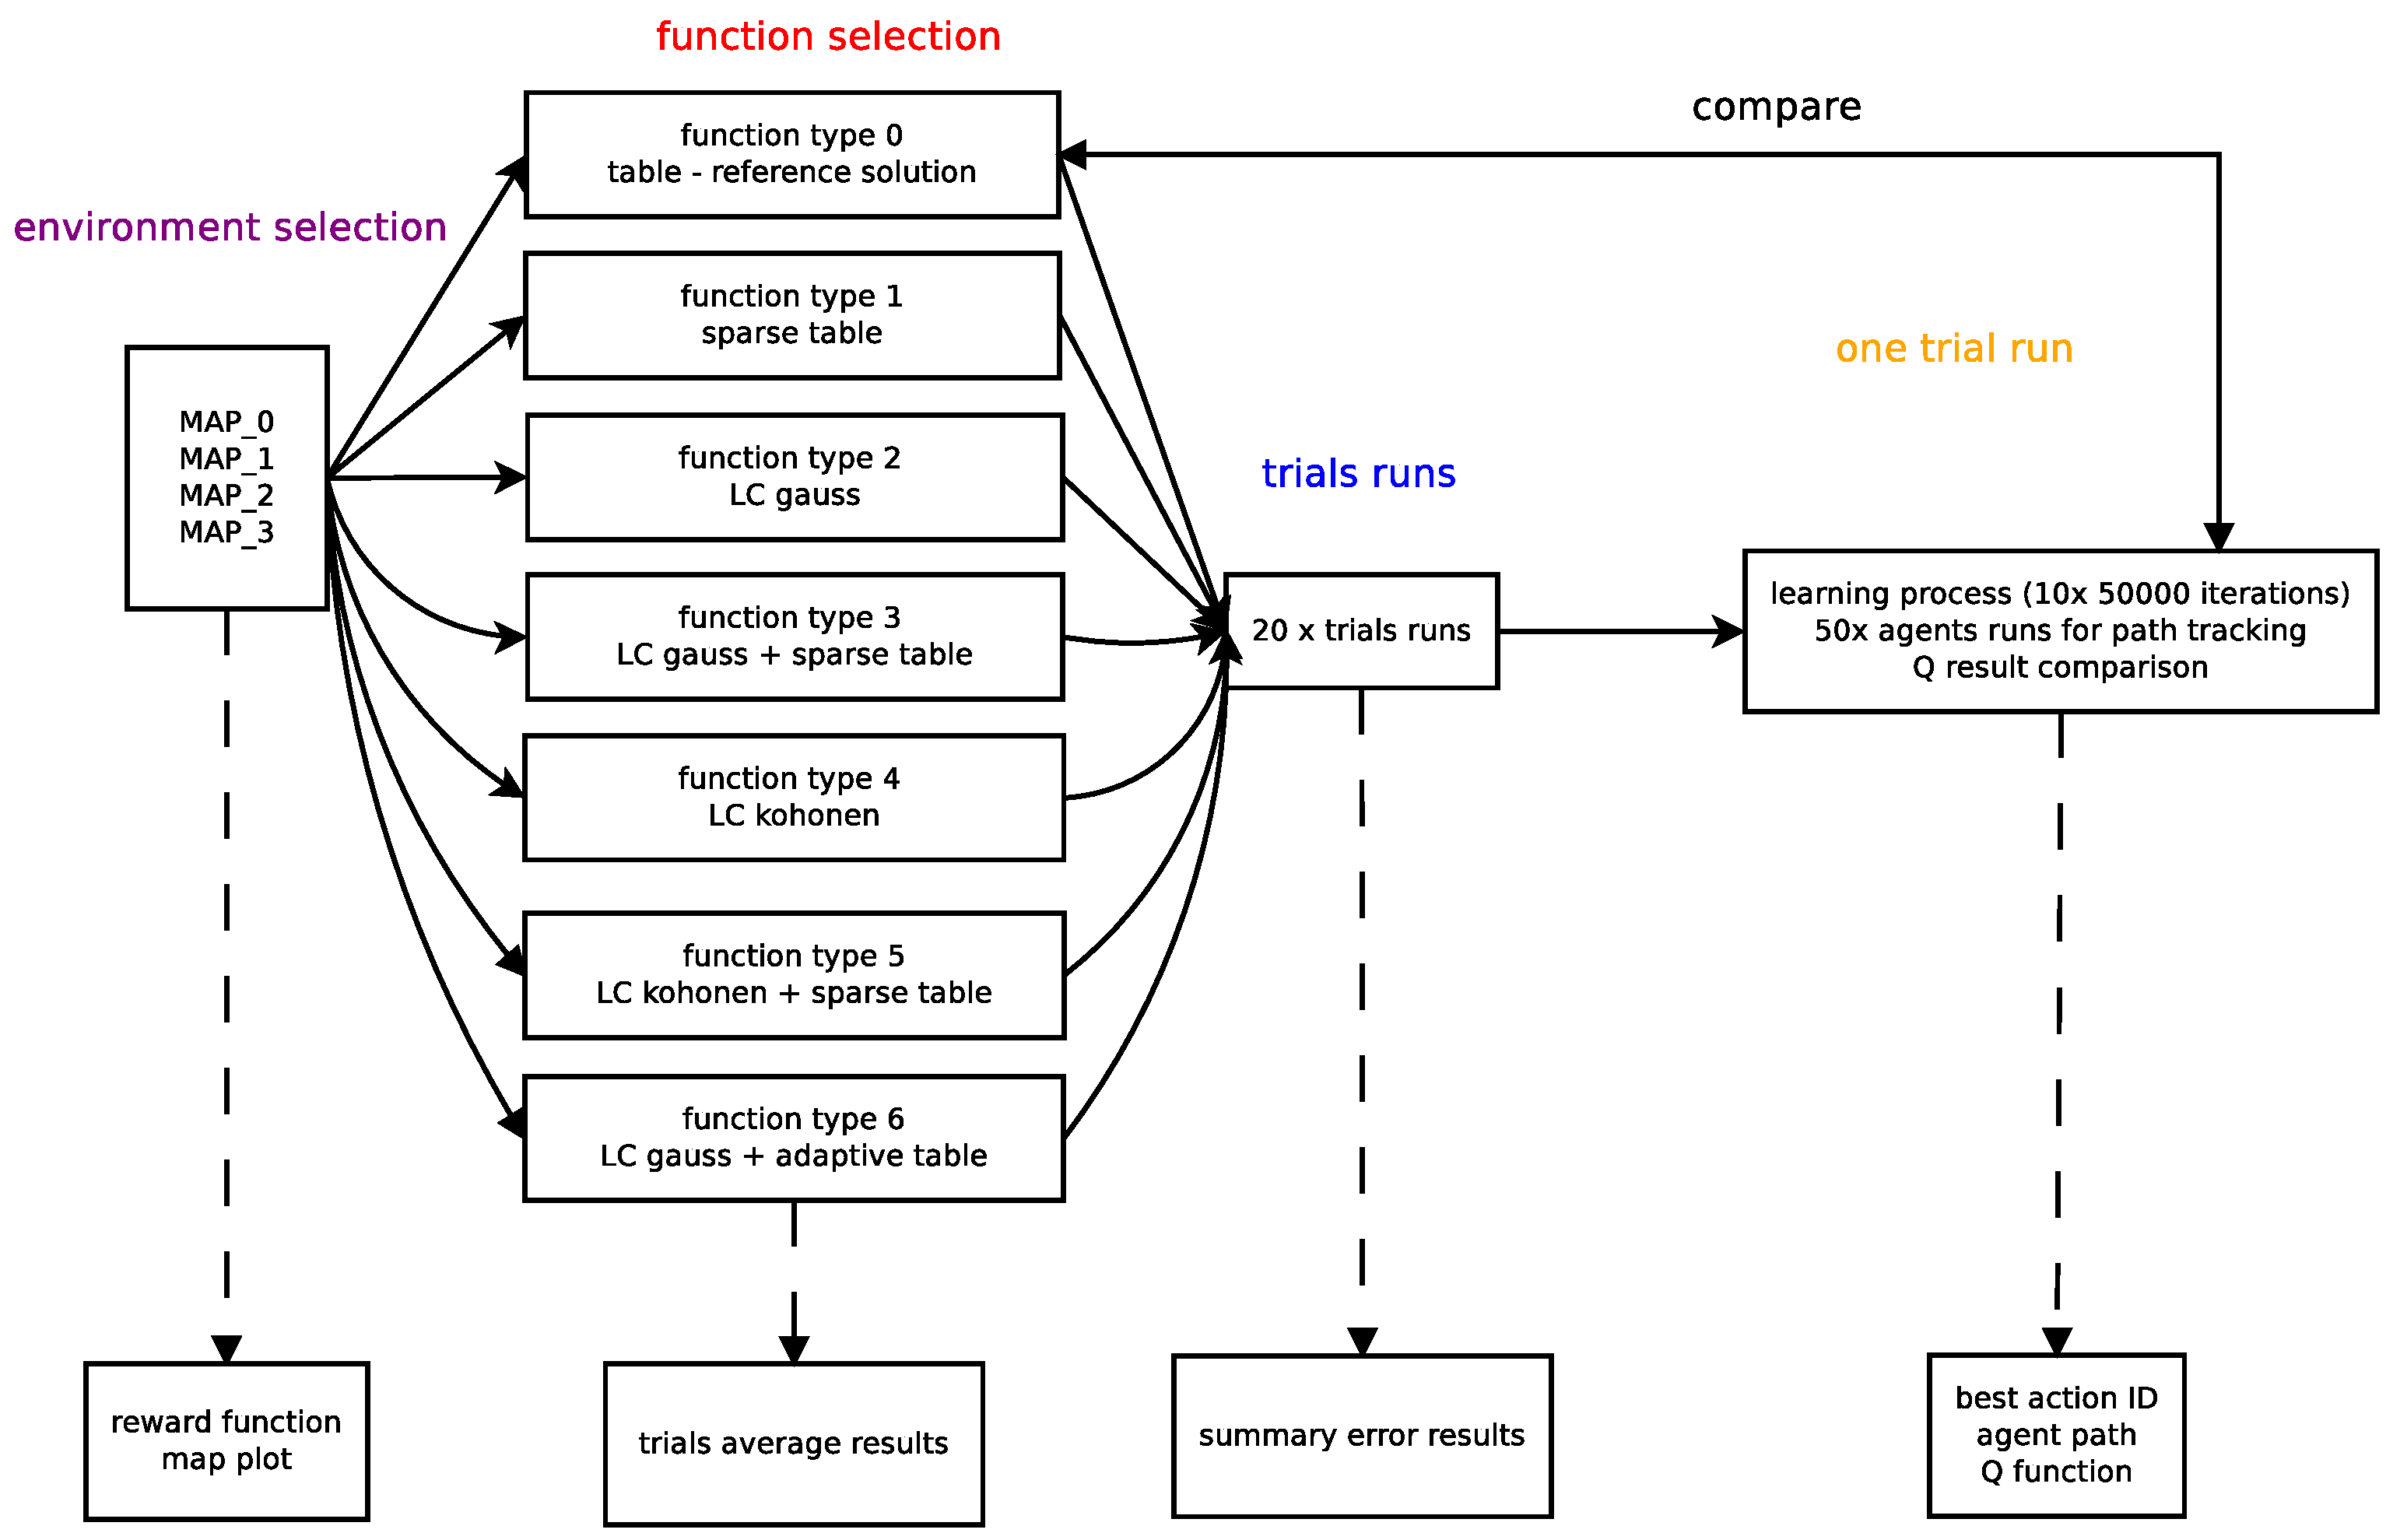
\includegraphics[scale=.3]{../diagrams/experiment_map_q_learning.eps}
\caption{Schéma experimentu}
\label{img:experiment_schem}
\end{figure}

Súhrnná schéma behu experimentov je na obrázku \ref{img:experiment_schem}.
Plné šípky predstavujú prepojenie úrovni metodológie. Čiarkované šípky znázorňujú
výstupy v jednotlivých úrovniach. Presné riešenie je použité na porovnanie výslednej chyby.



\begin{itemize}
\item 50000 iterácií učenia
\item rozmer $s$ je $n_s = 2$, rozmer $a$ je $n_a = 2$
\item predpis funkcie ohodnotení
\begin{align}
&Q(s(n),a(n)) = \nonumber \\
&\alpha Q(s(n-1),a(n-1)) \nonumber \\
&(1- \alpha)(R(s(n),a(n)) + \gamma \max_{a(n-1) \in \mathbb{A}} Q(s(n-1), a(n-1)) \nonumber
\end{align}

\item $R(s(n), a(n)) \in \langle -1, 1 \rangle$ náhodná mapa s 1 cieľovým stavom
\item $\gamma = 0.98$ a $\alpha = 0.7$
\item hustota referenčného riešenia = 1/32  (4096 stavov)
\item počet akcií v každom stave = 8
\item hustota riedkej tabuľky = 1/8  (1:16 pomer)
\item počet bázických funkcií $l = 64$
\item rozsah parametrov
    \begin{itemize}
      \item $\alpha_{ja}(n) \in \langle -1, 1 \rangle$
      \item $\beta_{ja}(n) \in \langle 0, 200 \rangle$
      \item $w_{ja}(n) \in \langle -4, 4 \rangle$
    \end{itemize}
\end{itemize}

$Q_{rt}(s(n),a(n))$ referenčná funkcia Q (funkcia 0), kde $t \in \langle 0, 19 \rangle $ je číslo trialu  \\
$Q_{jt}(s(n),a(n))$ testované funkcie Q a $j \in \langle 1, 5 \rangle $. \\

Celková chyba behu trialu $t$ je \\
\begin{equation}
e_{jt} = \sum\limits_{s, a}{(Q_{rt}(s,a) - Q_{jt}(s,a))^2}  \nonumber
\end{equation}

priemerná, minimálna, maximálna chyba a smerodatná odchylka \\
\begin{align}
\bar{a_j} &= \frac{1}{20}\sum\limits_{t}{e_{jt}}  \nonumber \\
{e^{min}_j} &= \min_{t}{e_{jt}}  \nonumber \\
{e^{max}_j} &= \max_{t}{e_{jt}}  \nonumber \\
{\sigma_j}^2 &= \frac{1}{20}\sum\limits_{t}{(\bar{a_j} - e_{jt})^2}  \nonumber
\end{align}

\section {Výsledky experimentu}

Experiment bol spočítaný pre 4 rôzne mapy - funkcie $R(s(n), a(n))$. Je potrebné
poznamenať, že takto navrhnuté prostredie umožňuje agentovi aby nastala
každý možný stav - to komplikuje možnosť redukcie počtu stavov. Ukážka mapy č. 2
je na obrázku \ref{img:experiment_reward_function}. Pričom ako bolo v predošlej
časti povedané, platí $R^k(s(n), a(n)) = R^k(s(n))$, t.j. odmena je rovnaká v každom
prechode vedúcom do rovnakého stavu.

\begin{figure}[!htb]
\centering
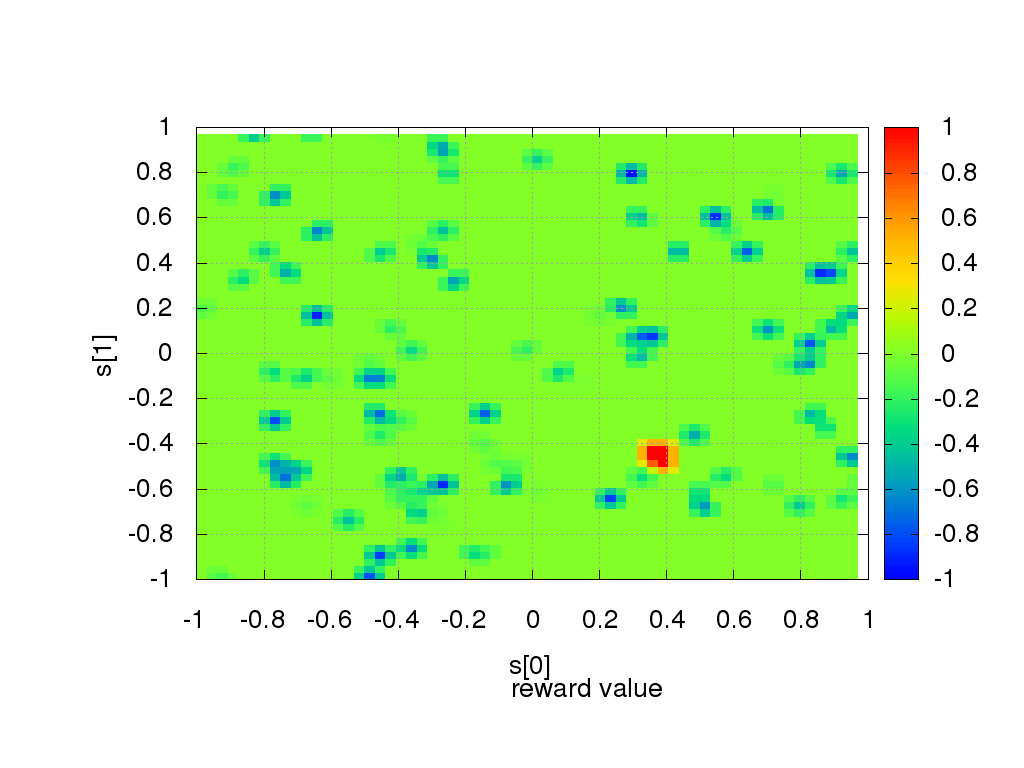
\includegraphics[scale=.4]{../../results_q_learning/map_2/reward_value_surface.png}
\caption{Odmeňovacia funkcia R(s(n), a(n)), mapa 2}
\label{img:experiment_reward_function}
\end{figure}


Pre riešenie Q funkcie s použitím tabuľky, ktoré bude vzhľadom na podmienky experimentu presným
rieším je graf funkcie $\max_{a(n) \in \mathbb{A}} Q_{n}(s(n), a(n))$ na obrázku \ref{img:experiment_reference}.
Je možné ľahko pozorovať maximum v oblasti jediného kladného $R(s(n), a(n))$. Od tohto
maxima sa šíria hodnoty na celý definičný obor podľa vzťahu \ref{eq:q_learning}. Ďalej
je možné pozrovať záporné hodnoty, ktoré sa nešíria ďalej - predstavujú oblasti kde $R(s(n), a(n))$
nadobúda tiež záporné hodnoty. Na základe známeho $Q(s(n),a(n))$ je možné
zostaviť mapu ktorú akciu číslovanú 0 až 7 má agent zvoliť - mapa najlepších
akcií v danom stave je znázornená na obrázku \ref{img:experiment_reference_action}.

\begin{figure}[!htb]
\centering
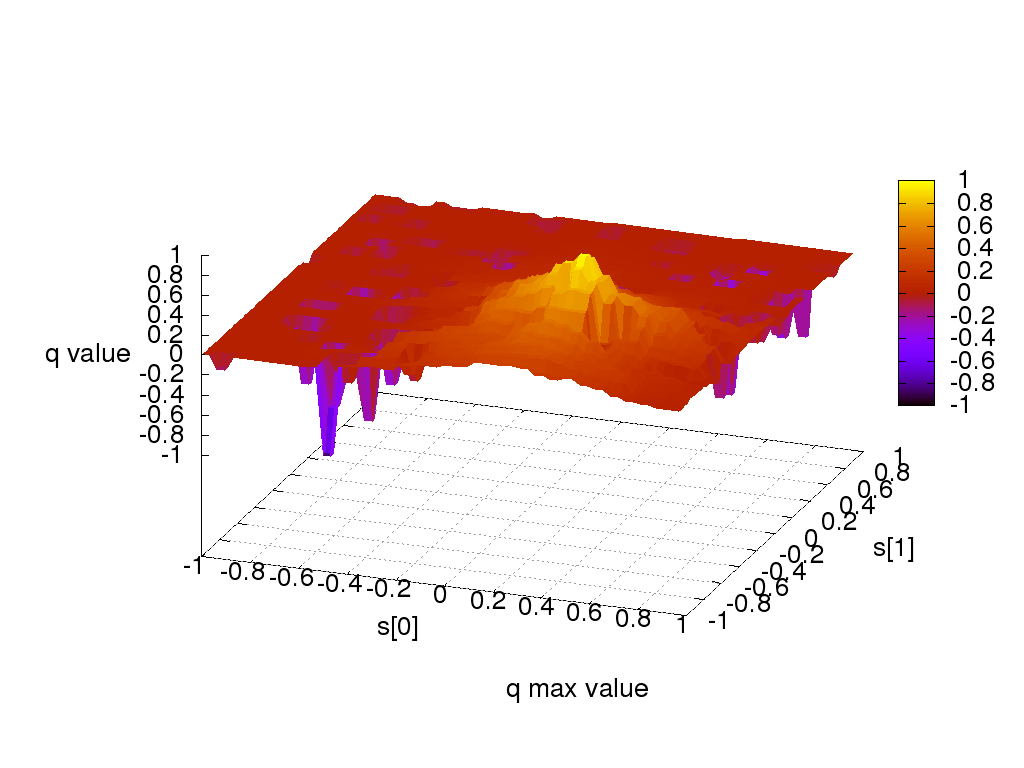
\includegraphics[scale=.4]{../../results_q_learning/map_2/function_type_0/iterations_10/q_learning_result.png}
\caption{Referenčné riešenie}
\label{img:experiment_reference}
\end{figure}

\begin{figure}[!htb]
\centering
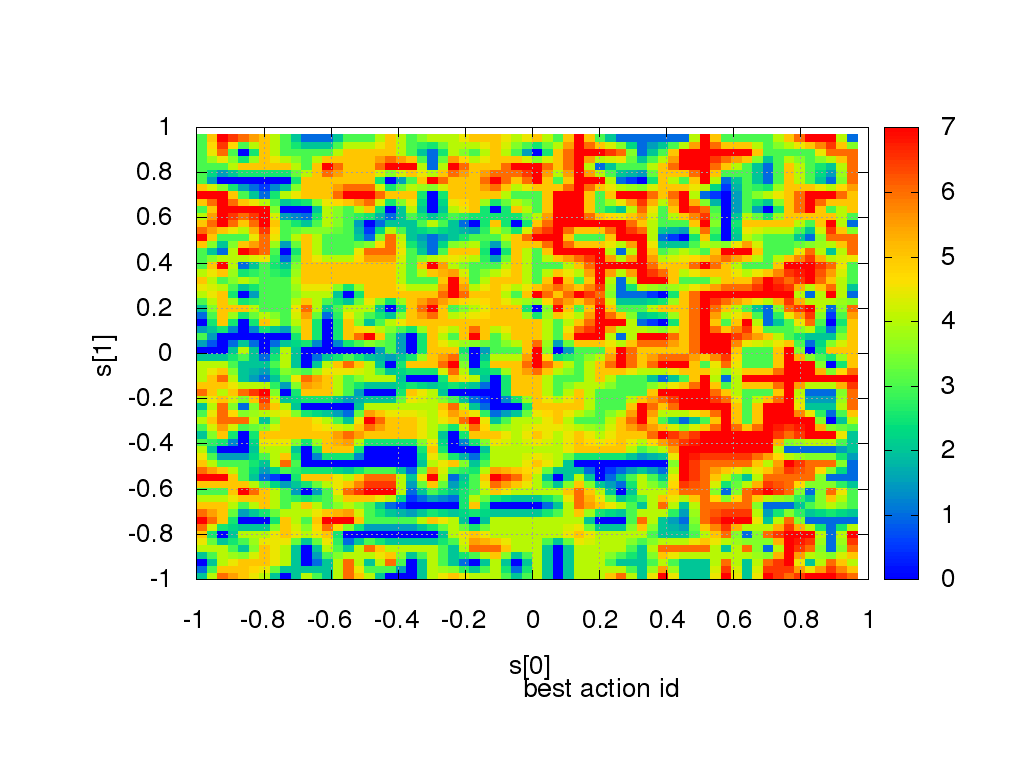
\includegraphics[scale=.4]{../../results_q_learning/map_2/function_type_0/iterations_10/action_best_value_log_surface.png}
\caption{Číslo najlepšej akcie použitím referenčného riešenia}
\label{img:experiment_reference_action}
\end{figure}

\newpage
Riešenie pre použitie riedkej tabuľky na aproximáciu je viditeľné na obrázku \ref{img:experiment_sparse_table}.
Je vidieť nespojité zmeny, a absenciu schopnosti aproximovať náhle záporné hodnoty požadované zápornou
$R(s(n), a(n))$. Zo známeho $Q(s(n), a(n))$ je ďalej možné zostaviť mapu najlepších akcií (očíslované od
0..7). Závislosť čísla najlepšej akcie od stavu je na obrázku \ref{img:experiment_sparse_table_actions}.


\begin{figure}[!htb]
\centering
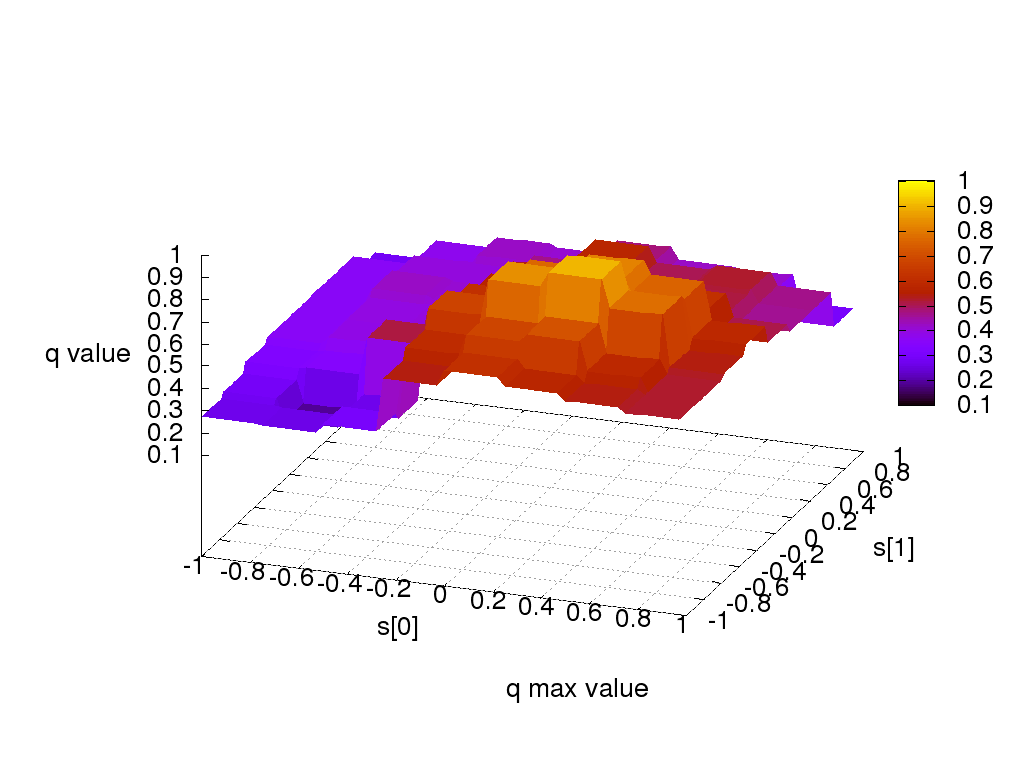
\includegraphics[scale=.4]{../../results_q_learning/map_2/function_type_1/iterations_10/q_learning_result.png}
\caption{Riešenie aproximácie použitím riedkej tabuľky}
\label{img:experiment_sparse_table}
\end{figure}


\begin{figure}[!htb]
\centering
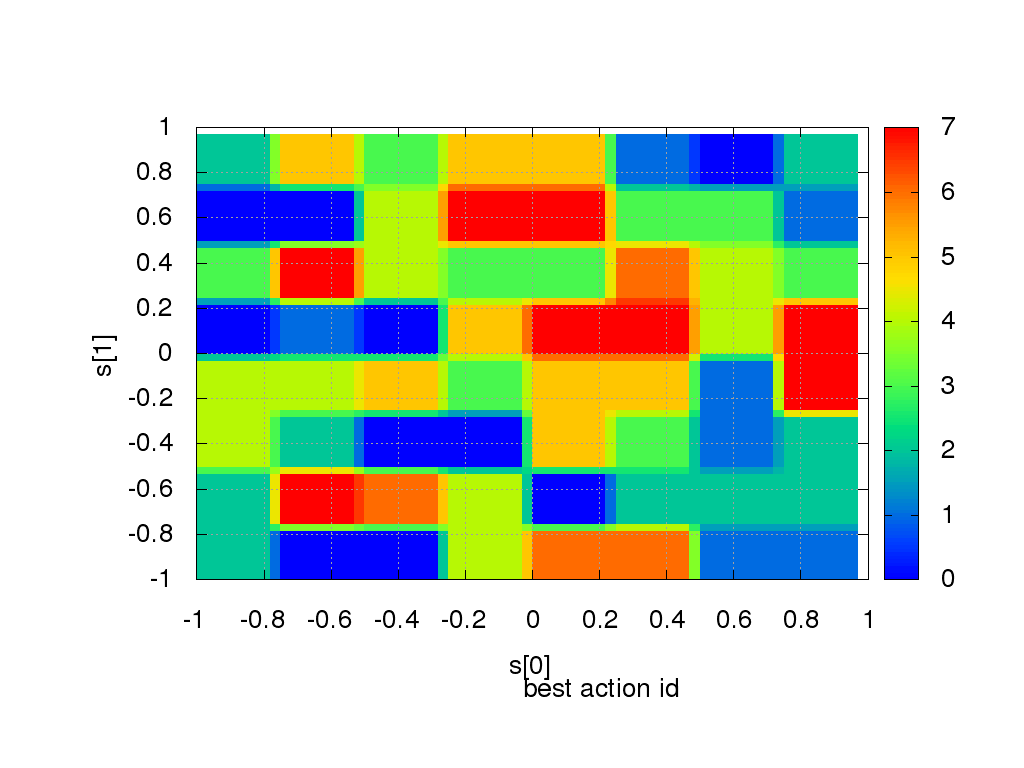
\includegraphics[scale=.4]{../../results_q_learning/map_2/function_type_1/iterations_10/action_best_value_log_surface.png}
\caption{Číslo Najlepšej akcie použitím riedkej tabuľky}
\label{img:experiment_sparse_table_actions}
\end{figure}

\newpage
Riešenie pre bázickú funkciu typu Gaussova krivka kombinovaná s riedkou tabuľkou (funkcia typu 3, obr. \ref{img:experiment_schem}) je na
obrázku \ref{img:experiment_gauss_sparse_table}. Je možné vidieť nepojité zmeny spôsobené riedkou tabuľkou
aj vyhladené oblasti vďaka Gaussovým krivkám. Podobne ako v predošlom prípade je možné znázorniť
závislosť najlepšej akcie od stavu na obrázku \ref{img:experiment_gauss_sparse_table_actions}. Oproti
riešeniu s riedkou tabuľkou je možné pozorovať zjemnenie prechodov.


\begin{figure}[!htb]
\centering
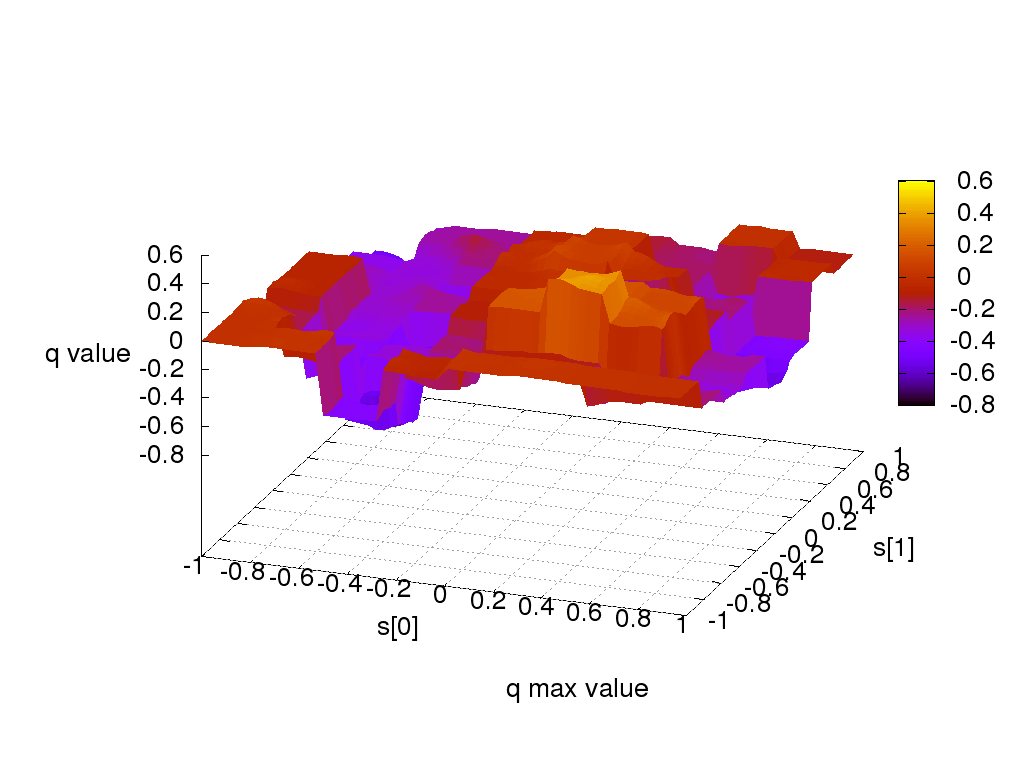
\includegraphics[scale=.4]{../../results_q_learning/map_2/function_type_3/iterations_10/q_learning_result.png}
\caption{Riešenie aproximácie použitím Gaussovej krivky kombinovanej s riedkou tabuľkou}
\label{img:experiment_gauss_sparse_table}
\end{figure}

\begin{figure}[!htb]
\centering
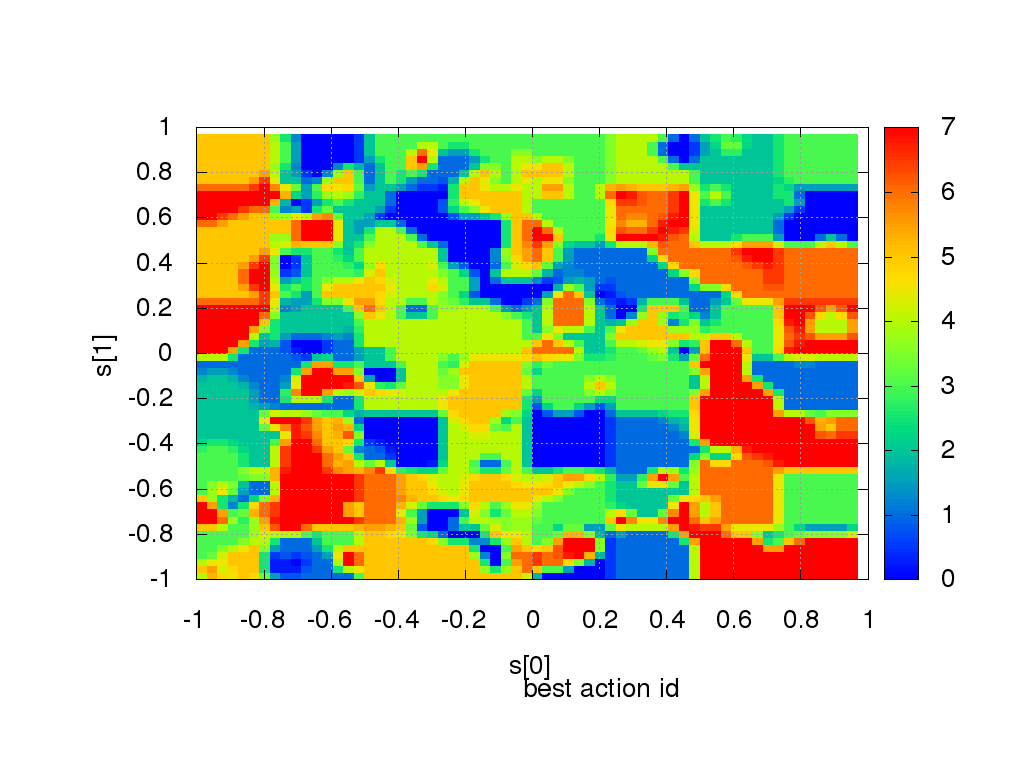
\includegraphics[scale=.4]{../../results_q_learning/map_2/function_type_3/iterations_10/action_best_value_log_surface.png}
\caption{Číslo najlepšej akcie použitím Gaussovej krivky kombinovanej s riedkou tabuľkou}
\label{img:experiment_gauss_sparse_table_actions}
\end{figure}

\newpage
Pre úplnosť, znázornenie riešenia pre novo zavedenú funkciu  \ref{eq:peak_hill} -
kombinujúc výhody hladkej Gaussovej krivky s tabuľkou, v bodoch kde sú záporné hodnoty $R(s(n), a(n))$.
Výsledok pre $\max_{a(n) \in \mathbb{A}} Q_{n}(s(n), a(n))$ je možné pozrovať na obrázku
\ref{img:experiment_gauss_adpative_table} a mapa najlepších akcií je na obrázku
\ref{img:experiment_gauss_adpative_table_actions}.


\begin{figure}[!htb]
\centering
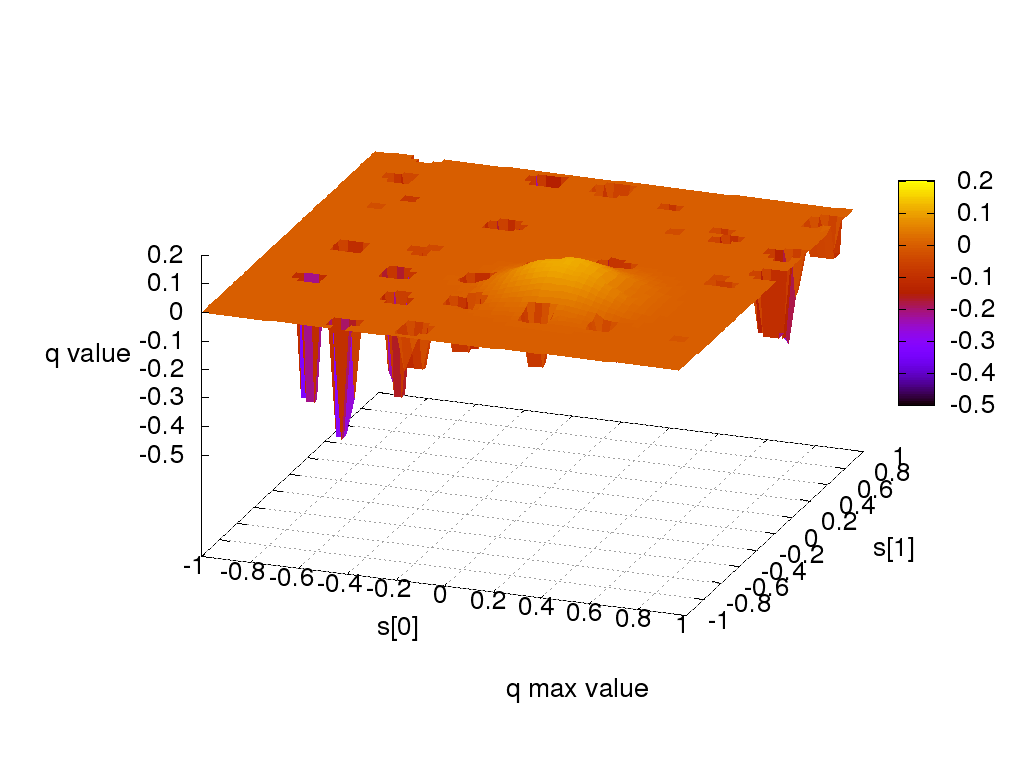
\includegraphics[scale=.4]{../../results_q_learning/map_2/function_type_6/iterations_10/q_learning_result.png}
\caption{Riešenie aproximácie použitím Gaussovej krivky kombinovanej s adaptívnou tabuľkou}
\label{img:experiment_gauss_adpative_table}
\end{figure}

\begin{figure}[!htb]
\centering
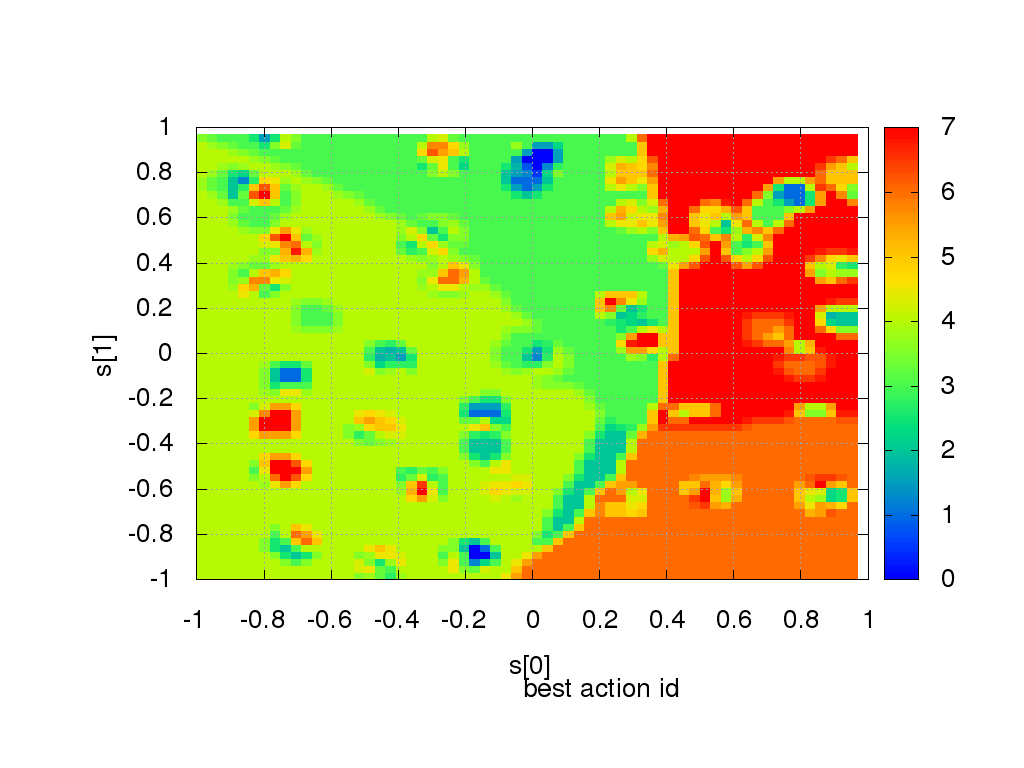
\includegraphics[scale=.4]{../../results_q_learning/map_2/function_type_6/iterations_10/action_best_value_log_surface.png}
\caption{Číslo najlepšej akcie použitím Gaussovej krivky kombinovanej s adaptívnou tabuľkou}
\label{img:experiment_gauss_adpative_table_actions}
\end{figure}


\newpage
\section {Priemerné výsledky experimentu}

V predošlej časti uvedené výsledky zobrazujú výsledne riešenia pre 3 zvolené aproximačné
metódy a jednu mapu - mapa 2. Celkové vyhodnotenie behu všetkých trialov a pre všetky
štyri mapy je na nasledujúcich obrázkoch. Sledovali sa veličiny priemerná, maximálna, minimálna chyba
a rozptyl chyby. Znázornenie výsledkov je na obrázkoch \ref{img:experiment_average_0},
\ref{img:experiment_average_1}, \ref{img:experiment_average_2} a \ref{img:experiment_average_3}.

\begin{figure}[!htb]
\centering
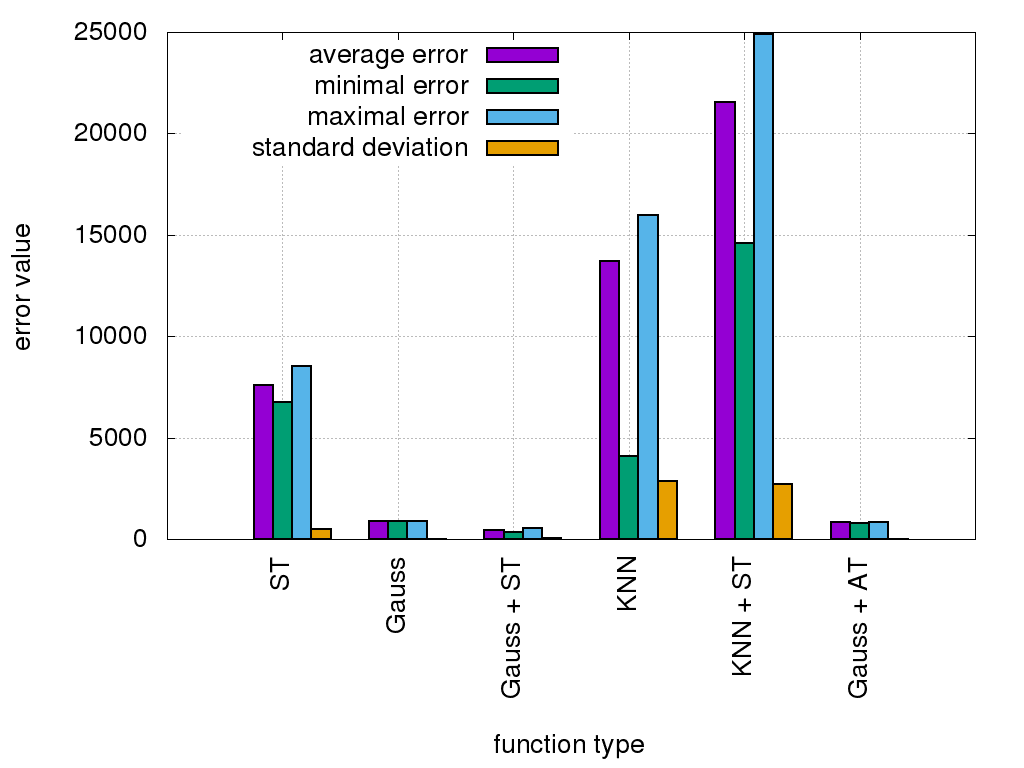
\includegraphics[scale=.4]{../../results_q_learning/map_0/trials_average_results.png}
\caption{Súhrnné výsledky pre všetky testovacie funkcie a mapu 0}
\label{img:experiment_average_0}
\end{figure}

\begin{figure}[!htb]
\centering
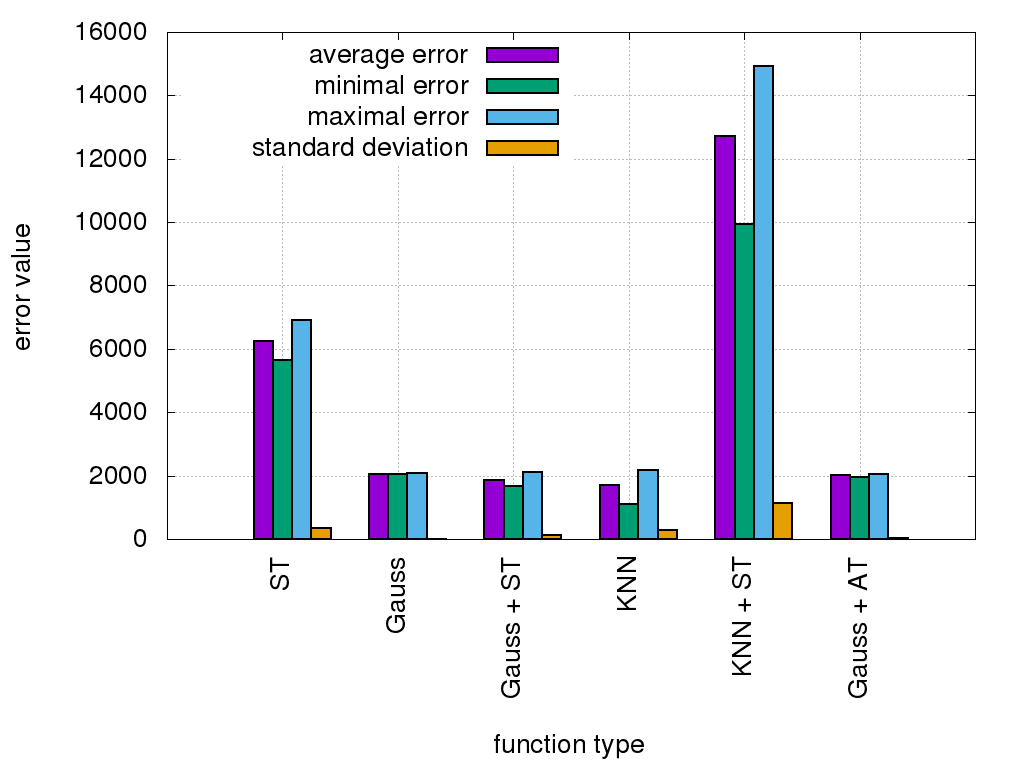
\includegraphics[scale=.4]{../../results_q_learning/map_1/trials_average_results.png}
\caption{Súhrnné výsledky pre všetky testovacie funkcie a mapu 1}
\label{img:experiment_average_1}
\end{figure}

\begin{figure}[!htb]
\centering
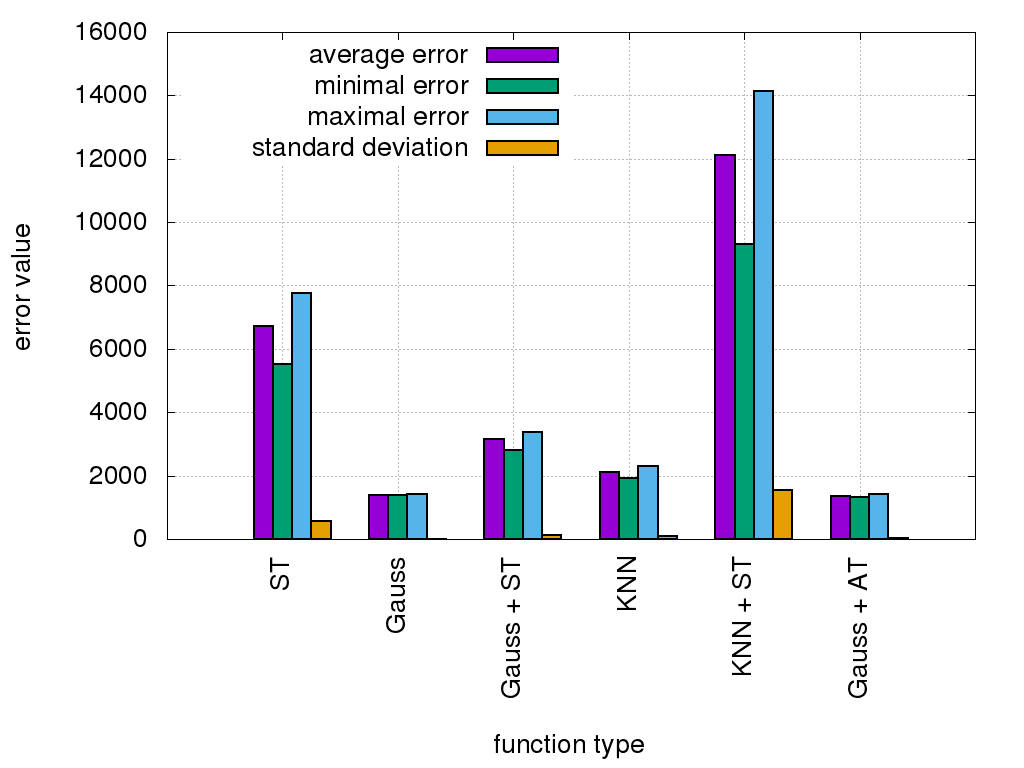
\includegraphics[scale=.4]{../../results_q_learning/map_2/trials_average_results.png}
\caption{Súhrnné výsledky pre všetky testovacie funkcie a mapu 2}
\label{img:experiment_average_2}
\end{figure}

\begin{figure}[!htb]
\centering
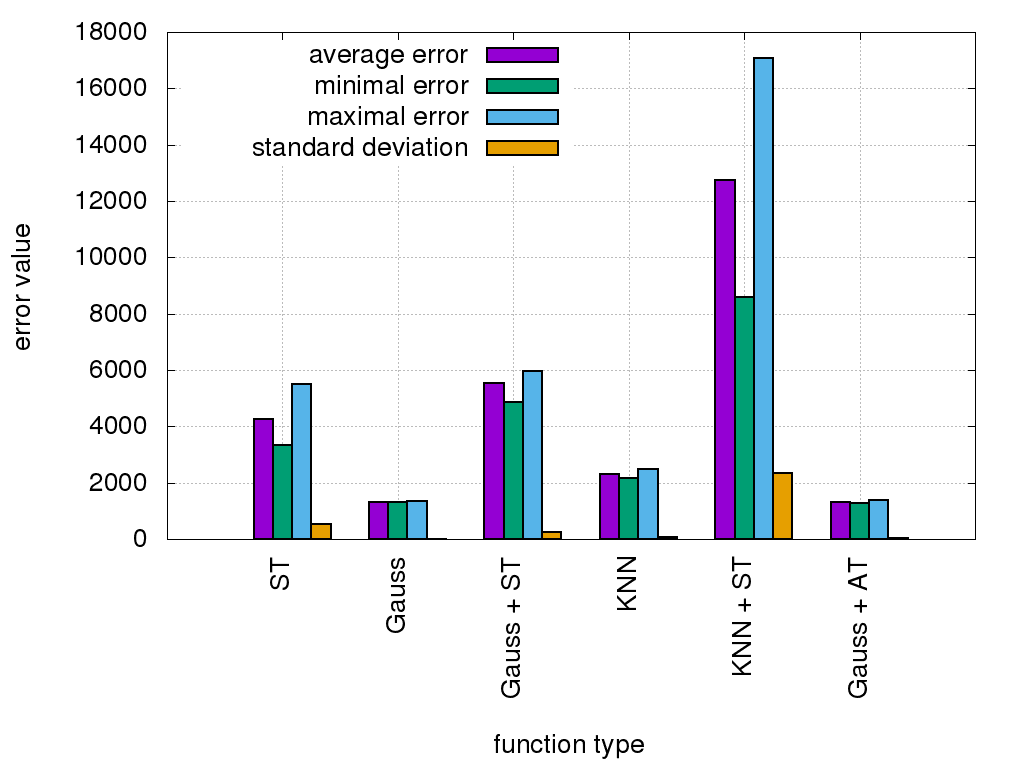
\includegraphics[scale=.4]{../../results_q_learning/map_3/trials_average_results.png}
\caption{Súhrnné výsledky pre všetky testovacie funkcie a mapu 3}
\label{img:experiment_average_3}
\end{figure}

Z výsledkov je možné vybrať troch najvhodnejších kandidátov na aproximáciu :
Gaussova krivka, Gaussova krivka kombinovaná s riedkou tabuľkou,
Gaussova krivka kombinovaná s adaptívnou tabuľkou. Výsledky sa môžu zdať
vyrovnané, dôležité je však znázroniť pohyby jednotlivých virtuálnych robotov a
podľa toho urobiť záver. Pohyby robotov pre mapu 2 a jednotlivé aproximačné
metódy je možné sledovať na obrázkoch
\ref{img:experiment_ref_path}
\ref{img:experiment_gauss_path}
\ref{img:experiment_gauss_sparse_table_path}
a   \ref{img:experiment_gauss_adaptive_table_path}. Je zrejmé, že jedina vyhovujúca
aproximačná metóda pre uvedené parametre experimentu je novo zavedená funkcia \ref{eq:peak_hill}.
Príčinou zlyhania ostatných je neschopnosť zebezpečiť potrebnú strmosť v oblastiach
zápornej hodnoty $R(s(n), a(n))$. Samotná rekurentná povaha Q-learning algoritmu spôsobuje,
že s rastúcou vzdialenosťou od jediného kladného $R(s(n), a(n))$ sa zmenšujú rozdiely
$Q(s(n), a(n))$ pre jednotlivé akcie ktoré je možné v danom stave vykonať. To je obzvlášť nepríjemne
pre experiment tak ako bol navrhnutý - malá zmena pohybu robota znamená aj malú zmenu stavu
a aproximačná funkcia tak veľmi ťažko zachytí zmenu s požadovanou presnosťou.


  \begin{figure}[!htb]
  \centering
  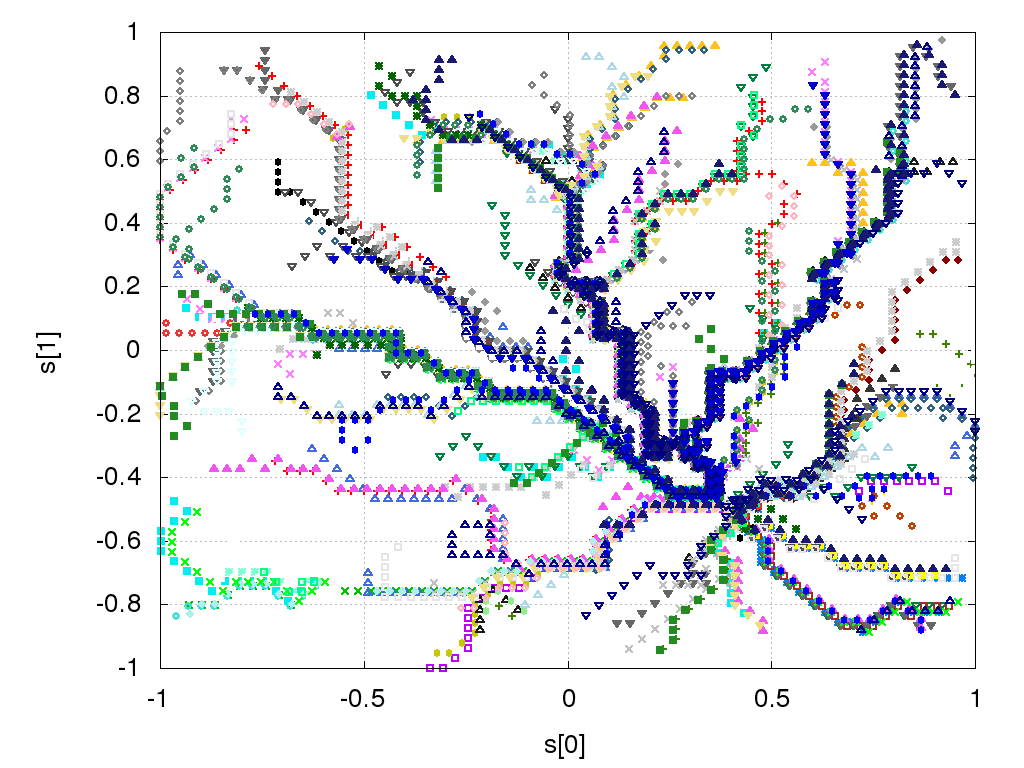
\includegraphics[scale=.4]{../../results_q_learning/map_2/function_type_0/iterations_10/agents_path_surface.png}
  \caption{Dráha robotov, referenčné riešenie}
  \label{img:experiment_ref_path}
  \end{figure}

  \begin{figure}[!htb]
  \centering
  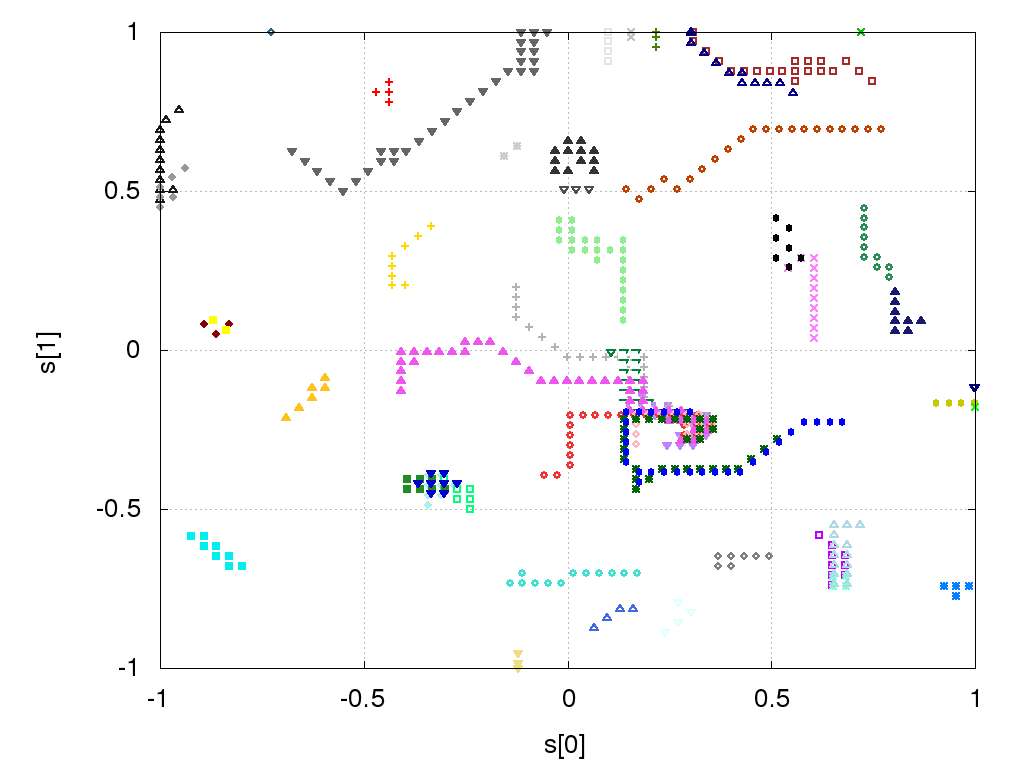
\includegraphics[scale=.4]{../../results_q_learning/map_2/function_type_2/iterations_10/agents_path_surface.png}
  \caption{Dráha robotov, aproximacia  Gaussovou krivkou}
  \label{img:experiment_gauss_path}
  \end{figure}


  \begin{figure}[!htb]
  \centering
  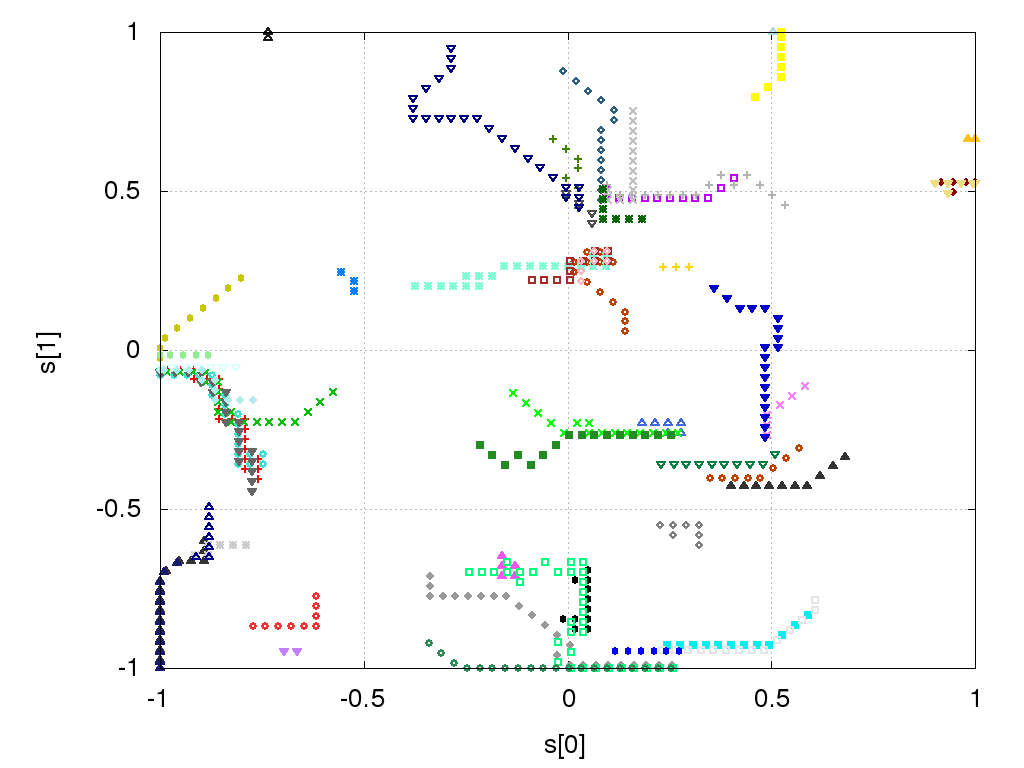
\includegraphics[scale=.4]{../../results_q_learning/map_2/function_type_3/iterations_10/agents_path_surface.png}
  \caption{Dráha robotov, aproximacia  Gaussovou krivkou kombinovanou s riedkou tabuľkou}
  \label{img:experiment_gauss_sparse_table_path}
  \end{figure}


  \begin{figure}[!htb]
  \centering
  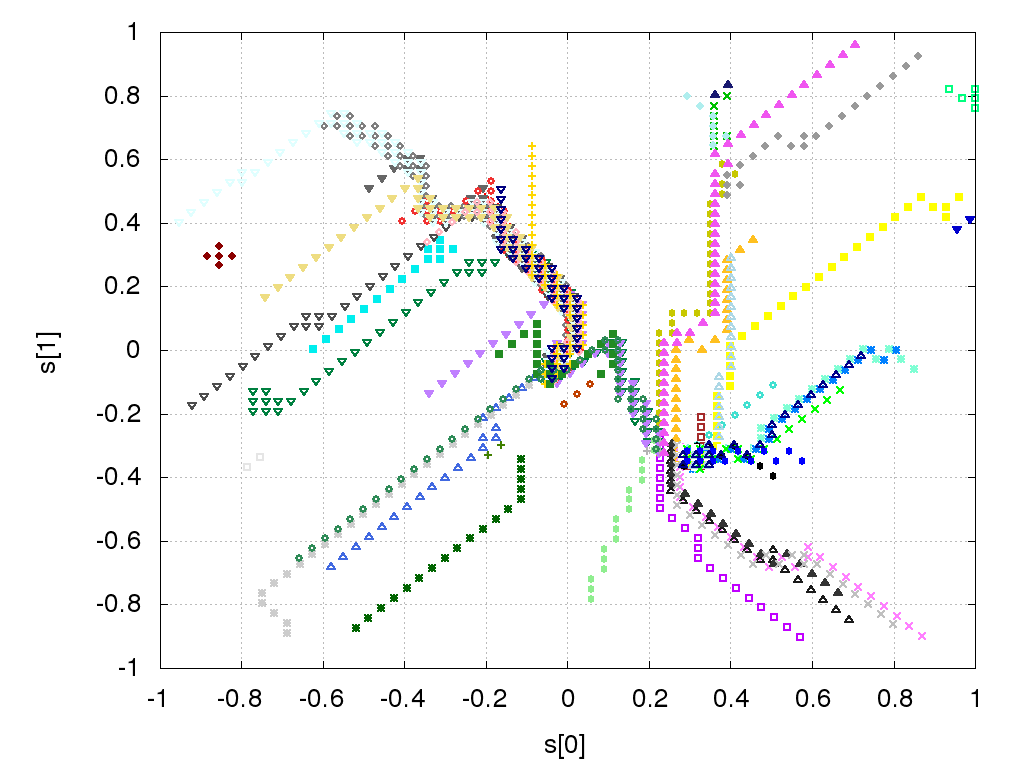
\includegraphics[scale=.4]{../../results_q_learning/map_2/function_type_6/iterations_10/agents_path_surface.png}
  \caption{Dráha robotov, aproximacia  Gaussovou krivkou kombinovanou s adaptívnou tabuľkou}
  \label{img:experiment_gauss_adaptive_table_path}
  \end{figure}
